\documentclass[10pt]{article}
\usepackage[margin=0.8in]{geometry}

\usepackage[utf8]{inputenc}
\usepackage[T1]{fontenc}
\usepackage{amsmath}
\usepackage{amsfonts}
\usepackage{amssymb}
\usepackage[version=4]{mhchem}
\usepackage{stmaryrd}
\usepackage{graphicx}
\usepackage[export]{adjustbox}
\usepackage{bbold}
\usepackage{fixltx2e}
\usepackage{caption}
\usepackage{mathtools}
\usepackage{amsfonts} %% <- also included by amssymb
\DeclareMathSymbol{-}{\mathbin}{AMSa}{"39}
\usepackage[parfill]{parskip}
	
\usepackage[framemethod=TikZ]{mdframed}
\colorlet{shadecolor}{orange!15}
\usepackage{xcolor}
\usepackage{amsthm}
\usepackage{framed}





\begin{document}

\title{Lecture 3-5: Basic Kinematics}
\date{Aug. 24, 2023 \quad  Aug. 29, 2023 \quad  Aug. 31, 2023}
\author{Wanxin Jin}
\maketitle




\section{Pose of a Rigid Body}
The pose of a rigid body in 3D space is  described  by its position and orientation with respect to a reference frame.  As shown in Fig. \ref{fig.rbpos},  let $O- x y z$ be the reference frame and $\{\boldsymbol{x}, \boldsymbol{y}, \boldsymbol{z}\}$ be the unit vectors of the frame axes. In order to represent the pose of the rigid body, we pick a fixed point $O^\prime$ on the rigid body, and attach an orthonormal body frame $O^{\prime} - x^{\prime} y^{\prime} z^{\prime}$  to the body, with origin in $O^{\prime}$. $\{\boldsymbol{x}^{\prime}, \boldsymbol{y}^{\prime}, \boldsymbol{z}^{\prime}\}$  are the unit vectors of the body frame axes, 

\begin{figure}[h]
    \centering
    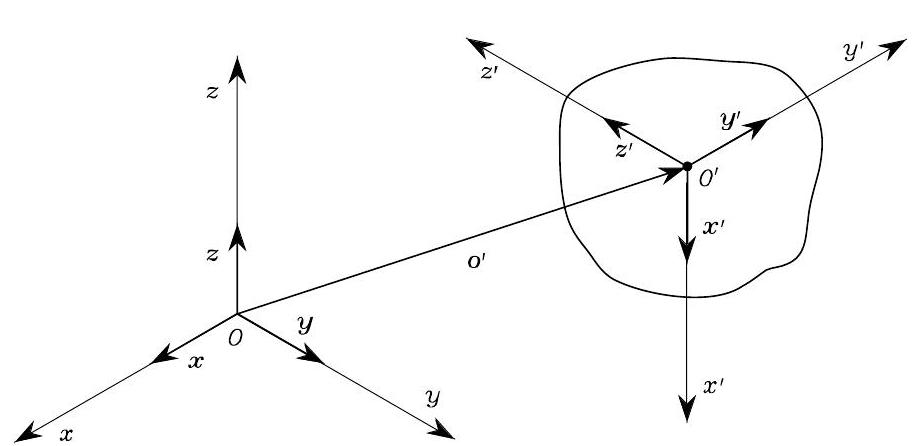
\includegraphics[max width=0.5\textwidth]{./kinematics/pose_rigid_body}
    \caption{Pose of a rigid body in a reference frame}
    \label{fig.rbpos}
\end{figure}



To describe the position of the rigid body, we define a position vector $\boldsymbol{o}^{\prime}$ pointing from the reference frame origin $O$ to the body frame origin $O'$. We express $\boldsymbol{o}^{\prime}$ in terms of $\{\boldsymbol{x}, \boldsymbol{y}, \boldsymbol{z}\}$ of reference frame:

$$
    \boldsymbol{o}^{\prime}=o_{x}^{\prime} \boldsymbol{x}+o_{y}^{\prime} \boldsymbol{y}+o_{z}^{\prime} \boldsymbol{z}
:=\left[\begin{array}{c}
o_{x}^{\prime} \\
o_{y}^{\prime} \\
o_{z}^{\prime}
\end{array}\right]
=\left[\begin{array}{c}
{\boldsymbol{o}^{\prime}}^T \boldsymbol{x} \\
{\boldsymbol{o}^{\prime}}^T \boldsymbol{y} \\
{\boldsymbol{o}^{\prime}}^T \boldsymbol{z}
\end{array}\right]
$$

where $o_{x}^{\prime}, o_{y}^{\prime}, o_{z}^{\prime}$ are  projections of   $\boldsymbol{o}^{\prime}$ in each axis in $\{\boldsymbol{x}, \boldsymbol{y}, \boldsymbol{z}\}$, and they are called the coordinates of the vector.

\smallskip

To describe the  orientation of the rigid body, we find the coordinates of each unit axis in $\{\boldsymbol{x}^{\prime}, \boldsymbol{y}^{\prime}, \boldsymbol{z}^{\prime}\}$ of rigid body frame, in terms of $\{\boldsymbol{x}, \boldsymbol{y}, \boldsymbol{z}\}$ of reference frame:

$$
    \begin{aligned}
& \boldsymbol{x}^{\prime}=x_{x}^{\prime} \boldsymbol{x}+x_{y}^{\prime} \boldsymbol{y}+x_{z}^{\prime} \boldsymbol{z} \\
& \boldsymbol{y}^{\prime}=y_{x}^{\prime} \boldsymbol{x}+y_{y}^{\prime} \boldsymbol{y}+y_{z}^{\prime} \boldsymbol{z} \\
& \boldsymbol{z}^{\prime}=z_{x}^{\prime} \boldsymbol{x}+z_{y}^{\prime} \boldsymbol{y}+z_{z}^{\prime} \boldsymbol{z} .
\end{aligned}
$$

Write the above into the following compact notation:

$$
    \boldsymbol{R}=\left[\begin{array}{lll}
\boldsymbol{x}^{\prime} & \boldsymbol{y}^{\prime} & \boldsymbol{z}^{\prime} 
\end{array}\right]=\left[\begin{array}{ccc}
x_{x}^{\prime} & y_{x}^{\prime} & z_{x}^{\prime} \\
x_{y}^{\prime} & y_{y}^{\prime} & z_{y}^{\prime} \\
x_{z}^{\prime} & y_{z}^{\prime} & z_{z}^{\prime}
\end{array}\right]=\left[\begin{array}{lll}
\boldsymbol{x}^{\prime T} \boldsymbol{x} & \boldsymbol{y}^{\prime T} \boldsymbol{x} & \boldsymbol{z}^{\prime T} \boldsymbol{x} \\
\boldsymbol{x}^{\prime T} \boldsymbol{y} & \boldsymbol{y}^{\prime T} \boldsymbol{y} & \boldsymbol{z}^{\prime T} \boldsymbol{y} \\
\boldsymbol{x}^{\prime T} \boldsymbol{z} & \boldsymbol{y}^{\prime T} \boldsymbol{z} & \boldsymbol{z}^{T} \boldsymbol{z}
\end{array}\right]
$$

with each column being  the coordinates of each unit vector in $\{\boldsymbol{x}^{\prime}, \boldsymbol{y}^{\prime}, \boldsymbol{z}^{\prime}\}$. The  $\boldsymbol{R}$ is called rotation matrix. Some properties of Rotation Matrix include
\begin{itemize}
    \item Mutual orthogonality:
    $
\boldsymbol{x}^{\prime T} \boldsymbol{y}^{\prime}=0$, $\boldsymbol{y}^{\prime T} \boldsymbol{z}^{\prime}=0$, and $\boldsymbol{z}^{\prime T} \boldsymbol{x}^{\prime}=0$

    \item Unity: $\boldsymbol{x}^{\prime T} \boldsymbol{x}^{\prime}=1$, $\boldsymbol{y}^{\prime T} \boldsymbol{y}^{\prime}=1$, and $\boldsymbol{z}^{\prime T} \boldsymbol{z}^{\prime}=1$

 \item Orthogonal matrix: $\boldsymbol{R}^{T} \boldsymbol{R}=\boldsymbol{I}_{3} \quad \rightarrow \quad \boldsymbol{R}^{T}=\boldsymbol{R}^{-1}$

 \item The determinant of $\boldsymbol{R}$: $\det \boldsymbol{R}=1$


\end{itemize}



\section{Elementary Rotations}
Consider the origin of the body frame coincides with the origin of the reference frame. The orientation of a body frame can be obtained via  rotations of the reference frame about coordinate axes. Below, we consider right-handed rotation convention:  rotations are positive if counter-clockwise about a axis. 


\begin{figure}[h]
    \centering
    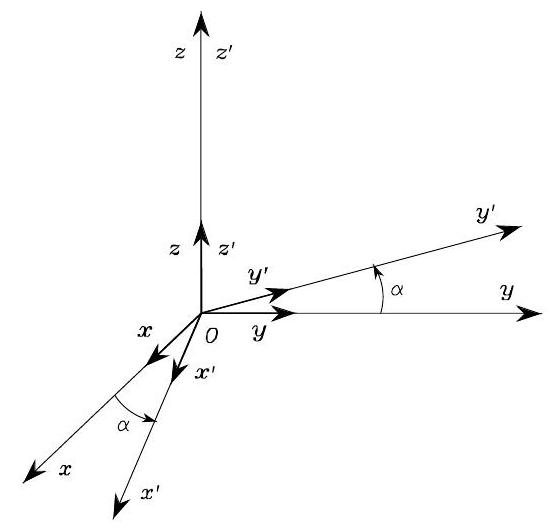
\includegraphics[max width=0.3\textwidth]{./kinematics/elementary_rotations}
    \caption{ Rotation of frame $O- x y z$ by an angle $\alpha$ about axis $\boldsymbol{z}$}
    \label{c1.rotation1}
\end{figure}





As shown in Fig. \ref{c1.rotation1}, suppose the body frame $O- x^{\prime} y^{\prime} z^{\prime}$ is a result of rotating  a reference frame $O- x y z$   by an angle $\alpha$ about the axis $\boldsymbol{z}$.  Then, the rotation matrix of $O- x^{\prime} y^{\prime} z^{\prime}$ is

$$
\boldsymbol{R}_{z}(\alpha)=\left[\begin{array}{lll}
\boldsymbol{x}^{\prime} & \boldsymbol{y}^{\prime} & \boldsymbol{z}^{\prime} 
\end{array}\right]=\left[\begin{array}{ccc}
\cos \alpha & -\sin \alpha & 0 \\
\sin \alpha & \cos \alpha & 0 \\
0 & 0 & 1
\end{array}\right]
$$

Similarly,  the rotation matrix for an angle $\beta$ about axis $\boldsymbol{y}$ is

$$
\boldsymbol{R}_{y}(\beta)  =\left[\begin{array}{ccc}
\cos \beta & 0 & \sin \beta \\
0 & 1 & 0 \\
-\sin \beta & 0 & \cos \beta
\end{array}\right]
$$

and the rotation matrix for an angle $\gamma$ about axis $\boldsymbol{x}$ is


$$
\boldsymbol{R}_{x}(\gamma)  =\left[\begin{array}{ccc}
1 & 0 & 0 \\
0 & \cos \gamma & -\sin \gamma \\
0 & \sin \gamma & \cos \gamma
\end{array}\right] .
$$

\emph{Takeaway: the rotation matrix can be interpreted geometrically as a rotation about an axis in space needed to align a reference frame to a body frame.}

\section{Transformation via Rotation Matrix}

\subsection{Passive Rotation}
Consider that the origin of the body frame coincides with the origin of the reference frame, and that a  point $P$ in space expressed in $O- x y z$ is

\begin{figure}[h]
    \centering
    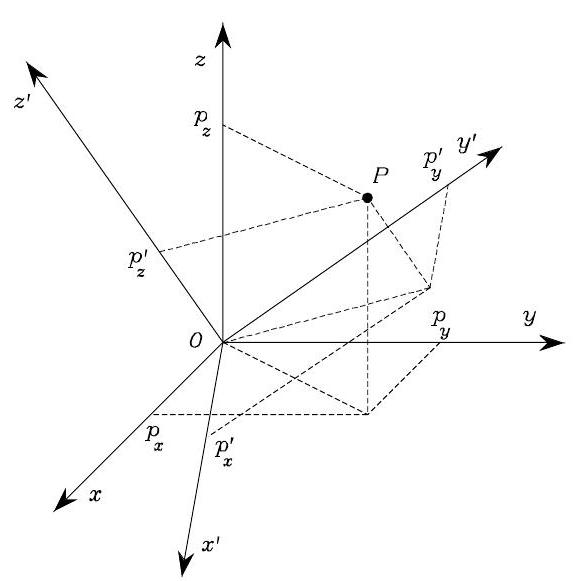
\includegraphics[max width=0.3\textwidth]{./kinematics/coordinate_transformation}
    \caption{Representation of a point $P$ in two different coordinate frames}
    \label{c1.rotation1}
\end{figure}


$$
\boldsymbol{p}=p_{x} \boldsymbol{x} +
p_{y} \boldsymbol{y} +
p_{z}\boldsymbol{z} 
=\left[\begin{array}{c}
p_{x} \\
p_{y} \\
p_{z}
\end{array}\right]
$$
The same point can also be expressed in $O- x^{\prime} y^{\prime} z^{\prime}$ as

$$
\boldsymbol{p}^{\prime}=p_{x}^{\prime} \boldsymbol{x}^{\prime} +
p_{y}^{\prime} \boldsymbol{y}^{\prime} +
p_{z}^{\prime}\boldsymbol{z}^{\prime} =\left[\begin{array}{c}
p_{x}^{\prime} \\
p_{y}^{\prime} \\
p_{z}^{\prime}
\end{array}\right]
$$



To establish the relationship between two coordinates, we need to replace the unite vectors $\{\boldsymbol{x}^{\prime}, \boldsymbol{y}^{\prime}, \boldsymbol{x}^{\prime}\}$ of the body frame with their coordinates in the reference frame using the rotation matrix  $\boldsymbol{R}$. This leads to

\begin{equation}\label{equ.transform}
    \boldsymbol{p}=\boldsymbol{R}\boldsymbol{p}^{\prime}
\end{equation}

\emph{Takeaway: $\boldsymbol{R}$ represents the transformation matrix of the coordinates in frame $O- x^{\prime} y^{\prime} z^{\prime}$ to the coordinates of the same vector in frame $O- x y z$. }




\subsection{Active Rotation}
In another perspective to look at (\ref{equ.transform}), we can interpret  $\boldsymbol{p}^{\prime}$ be a vector also in the reference frame $O- x y z$;  $\boldsymbol{R} \boldsymbol{p}^{\prime}$ yields a vector $\boldsymbol{p}$ with the same norm as that of $\boldsymbol{p}^{\prime}$ but rotated with respect to $\boldsymbol{p}^{\prime}$ according to the matrix $\boldsymbol{R}$.


\emph{Takeaway: $\boldsymbol{R}$ can be also interpreted as the matrix operator allowing rotation of a vector by a given angle about an axis in space.}






\section{Composition of Rotations}

\subsection{Rotation around Current Frame}

Let $O-{x_{0} y_{0} z_{0}}$, $O- x_{1} y_{1} z_{1}, O- x_{2} y_{2} z_{2}$ be three frames with common origin $O$. The same vector $\boldsymbol{p}$ can be expressed in each of the above frames, denoted as $\boldsymbol{p}^{0}, \boldsymbol{p}^{1}, \boldsymbol{p}^{2}$, respectively. Let $\boldsymbol{R}_{i}^{j}$ denote the rotation matrix of frame $i$ w.r.t. frame $j$.
One has

$$
\boldsymbol{p}^{1}=\boldsymbol{R}_{2}^{1} \boldsymbol{p}^{2}, \quad \boldsymbol{p}^{0}=\boldsymbol{R}_{1}^{0} \boldsymbol{p}^{1}, \quad \boldsymbol{p}^{0}=\boldsymbol{R}_{2}^{0} \boldsymbol{p}^{2}
$$

From the above  equations, one can derive

$$
\boldsymbol{R}_{2}^{0}=\boldsymbol{R}_{1}^{0} \boldsymbol{R}_{2}^{1}
$$

which is the composition of two rotations.  $\boldsymbol{R}_{2}^{0}$ can be thought of as  first rotating $O- x_{0} y_{0} z_{0}$ to $O- x_{1} y_{1} z_{1}$, according to $\boldsymbol{R}_{1}^{0}$, and then rotating $O- x_{1} y_{1} z_{1}$ to $O - x_{2} y_{2} z_{2}$, according to $\boldsymbol{R}_{2}^{1}$. Here, the first rotation matrix $\boldsymbol{R}_{1}^{0}$ is expressed in $O- x_{0} y_{0} z_{0}$, and the second rotation matrix $\boldsymbol{R}_{2}^{1}$ is expressed in $O- x_{1} y_{1} z_{1}$. 

Hence, we can conclude the following \emph{postmultiplication rule}:

\begin{itemize}
    \item The  frame with respect to which a rotation occurs (and the rotation matrix is `expressed') is called the current frame.
    \item The composition of each  rotation around  the current frame is  obtained by \emph{postmultiplication} of the rotation matrices in  order.
\end{itemize}



\subsection{Rotation around Fixed Frame}
Let's consider the following case. Suppose that we first rotate $O- x_{0} y_{0} z_{0}$ to frame $O- x_{1} y_{1} z_{1}$, according to $\boldsymbol{R}_{1}^{0}$ (which is expressed in the initial frame $O- x_{0} y_{0} z_{0}$). Next, we rotate the current frame $O- x_{1} y_{1} z_{1}$ to the frame $O- x_{2} y_{2} z_{2}$,  according to a new rotation matrix

$$
\boldsymbol{R}_{1,2}^0
$$

which is `expressed' \emph{still} in the initial frame $O- x_{0} y_{0} z_{0}$ (instead of the current frame $O- x_{1} y_{1} z_{1}$ itself). We call this type of rotation "the rotation around the fixed frame".




\smallskip
To apply the \emph{postmultipcation rule}, we need to find out the equivalent rotation to $\boldsymbol{R}_{1,2}^0$ but `expressed' in the current frame  $O- x_{1} y_{1} z_{1}$. This will lead to the concept of similarity transformation derived using the perspective of "rotation matrix as a active transformation" (how?).

\medskip

%Theorem
\begin{shaded}
Given a rotation matrix $\boldsymbol{R}^0$ `expressed' in the frame  $O- x_{0} y_{0} z_{0}$, the equivalent rotation matrix $\boldsymbol{R}^1$ `expressed' in another frame $O- x_{1} y_{1} z_{1}$, where $O- x_{1} y_{1} z_{1}$ is rotated by $\boldsymbol{R}_1^0$ from $O- x_{0} y_{0} z_{0}$ is 

$$
\boldsymbol{R}^1=(\boldsymbol{R}_1^0)^T\boldsymbol{R}^0\boldsymbol{R}_1^0
$$

\end{shaded}


Back to the matrix $\boldsymbol{R}_{1,2}^0$, the equivalent rotation matrix `expressed' in the  current frame  $O- x_{1} y_{1} z_{1}$ is 

$$
\boldsymbol{R}_{1,2}^1=(\boldsymbol{R}_1^0)^T\boldsymbol{R}_{1,2}^0\boldsymbol{R}_1^0
$$

Then, following the \emph{postmultipcation rule}, we can follow the   to obtain the total rotation
$$
\boldsymbol{R}_{2}^{0}=\boldsymbol{R}_{1}^{0} \boldsymbol{R}_{1,2}^1=\boldsymbol{R}_{1}^{0} (\boldsymbol{R}_1^0)^T\boldsymbol{R}_{1,2}^0\boldsymbol{R}_1^0=\boldsymbol{R}_{1,2}^0\boldsymbol{R}_1^0
$$


Hence, we can conclude the following \emph{premultiplication rule}:

\begin{itemize}
    \item The same frame with respect to which a rotation occurs (and the rotation matrix is `expressed') is called the fixed frame.
    \item The composition of each  rotation around  the fixed frame is  obtained by \emph{premultiplication} of the rotation matrices in  order.
\end{itemize}



Note: composition of rotations not commutative!


\section{Rotation Parameterization}
A rotation matrix has 9 elements, its mutual orthogonality and unity properties bring 6 constraints. Thus, 
only three independent parameters can minimally and sufficiently parameterize a rotation matrix.




\subsection{Euler Angles}


A rotation in space can be understood as a sequence of three elementary rotations. To fully describe all possible orientations, two successive rotations should not be made around parallel axes. When the first and third rotations are made around the same axis, the parameterization is called proper Euler angles. 
In the following, two sets of Euler angles are used; namely, the ZYZ Euler angles and the RPY (or Roll-PitchYaw) Euler angles.

\begin{figure}[h]
    \centering
    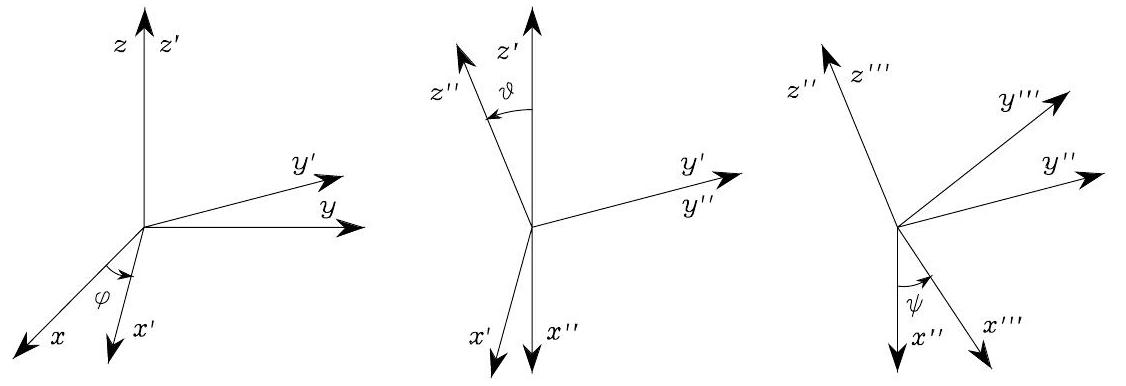
\includegraphics[max width=0.6\textwidth]{./kinematics/zyz_euler_angles}
    \caption{Parameterization of ZYZ Euler angles }
    \label{c1.fig.euler_angle_zyz}
\end{figure}


\bigskip
\noindent
\textbf{ZYZ Euler Angles}: the rotation described by ZYZ Euler angles is done by first,  rotating the current frame by  $\varphi$ about axis $\boldsymbol{z}$, second, rotating the current frame by  angle $\vartheta$ about axis $\boldsymbol{y}^{\prime}$, and then, rotating the current frame by the angle $\psi$ about axis $\boldsymbol{z}^{\prime\prime}$. Thus, 
the  rotation matrix from ZYZ Euler angles $\boldsymbol{\phi}=\left[\begin{array}{lll}\varphi & \vartheta & \psi\end{array}\right]^{T}$ is

$$
    \begin{aligned}
\boldsymbol{R}(\boldsymbol{\phi}) & =\boldsymbol{R}_{z}(\varphi) \boldsymbol{R}_{y^{\prime}}(\vartheta) \boldsymbol{R}_{z^{\prime \prime}}(\psi) =\left[\begin{array}{ccc}
c_{\varphi} c_{\vartheta} c_{\psi}-s_{\varphi} s_{\psi} & -c_{\varphi} c_{\vartheta} s_{\psi}-s_{\varphi} c_{\psi} & c_{\varphi} s_{\vartheta} \\
s_{\varphi} c_{\vartheta} c_{\psi}+c_{\varphi} s_{\psi} & -s_{\varphi} c_{\vartheta} s_{\psi}+c_{\varphi} c_{\psi} & s_{\varphi} s_{\vartheta} \\
-s_{\vartheta} c_{\psi} & s_{\vartheta} s_{\psi} & c_{\vartheta}
\end{array}\right] .
\end{aligned}
$$


Inversely, given a rotation matrix

$$
\boldsymbol{R}=\left[\begin{array}{lll}
r_{11} & r_{12} & r_{13} \\
r_{21} & r_{22} & r_{23} \\
r_{31} & r_{32} & r_{33}
\end{array}\right] .
$$

the corresponding ZYZ Euler angles $\boldsymbol{\phi}=\left[\begin{array}{lll}\varphi & \vartheta & \psi\end{array}\right]^{T}$ is 


$$
\begin{aligned}
& \varphi=\operatorname{Atan} 2\left(r_{23}, r_{13}\right) \\
& \vartheta=\operatorname{Atan} 2\left(\sqrt{r_{13}^{2}+r_{23}^{2}}, r_{33}\right) \\
& \psi=\operatorname{Atan} 2\left(r_{32},-r_{31}\right) .
\end{aligned}
$$

 if $s_{\vartheta}=0$, i.e., $(r_{23}, r_{13})\not=(0,0)$; otherwise,  only the sum or difference of $\varphi$ and $\psi$ is determined (why?)


\bigskip
\noindent
\textbf{RPY  Euler Angles}: the rotation from RPY  Euler angles is obtained by first, rotating the reference frame by the angle $\varphi$ about the current axis $\boldsymbol{z}$ (roll), then,  rotating the current frame by $\vartheta$ about the fixed axis $\boldsymbol{y}$ (pitch), and then,  rotating the current frame by $\psi$ about fixed axis $\boldsymbol{x}$ (yaw). Thus, the resulting rotation matrix is obtained by  premultiplication rule.

 
 

$$
\begin{aligned}
\boldsymbol{R}(\boldsymbol{\phi}) & =\boldsymbol{R}_{z}(\varphi) \boldsymbol{R}_{y}(\vartheta) \boldsymbol{R}_{x}(\psi)  =\left[\begin{array}{ccc}
c_{\varphi} c_{\vartheta} & c_{\varphi} s_{\vartheta} s_{\psi}-s_{\varphi} c_{\psi} & c_{\varphi} s_{\vartheta} c_{\psi}+s_{\varphi} s_{\psi} \\
s_{\varphi} c_{\vartheta} & s_{\varphi} s_{\vartheta} s_{\psi}+c_{\varphi} c_{\psi} & s_{\varphi} s_{\vartheta} c_{\psi}-c_{\varphi} s_{\psi} \\
-s_{\vartheta} & c_{\vartheta} s_{\psi} & c_{\vartheta} c_{\psi}
\end{array}\right] .
\end{aligned}
$$

\bigskip
Inversely, given rotation matrix

$$
\boldsymbol{R}=\left[\begin{array}{lll}
r_{11} & r_{12} & r_{13} \\
r_{21} & r_{22} & r_{23} \\
r_{31} & r_{32} & r_{33}
\end{array}\right],
$$

the corresponding ZYX  Euler Angles is  

$$
\begin{aligned}
& \varphi=\operatorname{Atan} 2\left(r_{21}, r_{11}\right) \\
& \vartheta=\operatorname{Atan} 2\left(-r_{31}, \sqrt{r_{32}^{2}+r_{33}^{2}}\right) \\
& \psi=\operatorname{Atan} 2\left(r_{32}, r_{33}\right) .
\end{aligned}
$$

if $c_{\vartheta}\not=0$; otherwise,  only the sum or difference of $\varphi$ and $\psi$ can be determined.



\subsection{Angle Axis}
The angle-axis is a non-minimal implementation of rotations, which is defined by an angle $\vartheta$ and a rotation axis vector $\boldsymbol{r}=\left[r_{x}, r_{y},  r_{z}\right]^{T}$ (unit vector) in the reference frame $O- x y z$. 

\begin{figure}[h]
    \centering
   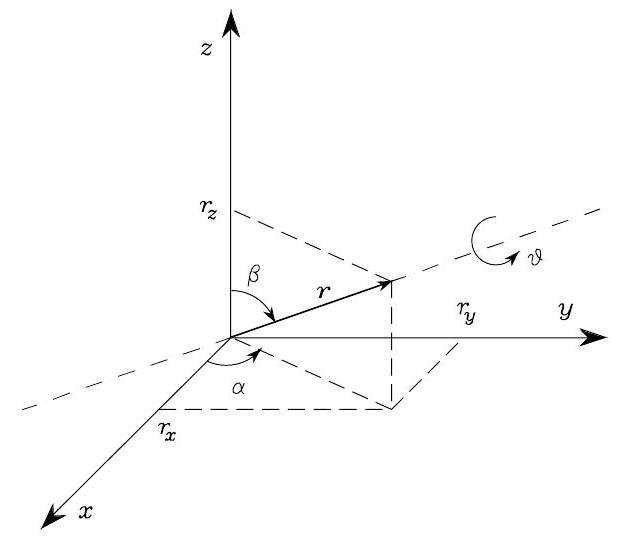
\includegraphics[max width=0.4\textwidth]{./kinematics/angle_axis}
    \caption{Rotation of an angle about an axis}
    \label{c1.fig.axis-angle}
\end{figure}



To derive the rotation matrix $\boldsymbol{R}(\vartheta, \boldsymbol{r})$ from $(\vartheta, \boldsymbol{r})$, we first create a `virtual' frame $O_1- x_1 y_1 z_1$ with its axis $\boldsymbol{z_1}$ aligned with $\boldsymbol{r}$. Then, the rotation matrix for the rotation $(\vartheta, \boldsymbol{r})$  is `expressed' in the current frame: $\boldsymbol{R}_{z}(\vartheta)$. Since our goal is to find the rotation matrix $\boldsymbol{R}(\vartheta, \boldsymbol{r})$  `expressed' in the reference frame $O- x y z$, we apply the previous similarity transformation: 

    $$
     \boldsymbol{R}(\vartheta, \boldsymbol{r})= \boldsymbol{R}_{b} \boldsymbol{R}_{z}(\vartheta) (\boldsymbol{R}_{b})^T
    $$

with $\boldsymbol{R}_{1}$ denoting the rotation from the reference frame to the virtual frame. From the geometry in Fig. \ref{c1.fig.axis-angle}, 

$$
\boldsymbol{R}_{b}=\boldsymbol{R}_{z}(\alpha) \boldsymbol{R}_{y}(\beta) 
$$


In sum, the rotation matrix is

$$
\boldsymbol{R}(\vartheta, \boldsymbol{r})=\left[\begin{array}{ccc}
r_{x}^{2}\left(1-c_{\vartheta}\right)+c_{\vartheta} & r_{x} r_{y}\left(1-c_{\vartheta}\right)-r_{z} s_{\vartheta} & r_{x} r_{z}\left(1-c_{\vartheta}\right)+r_{y} s_{\vartheta} \\
r_{x} r_{y}\left(1-c_{\vartheta}\right)+r_{z} s_{\vartheta} & r_{y}^{2}\left(1-c_{\vartheta}\right)+c_{\vartheta} & r_{y} r_{z}\left(1-c_{\vartheta}\right)-r_{x} s_{\vartheta} \\
r_{x} r_{z}\left(1-c_{\vartheta}\right)-r_{y} s_{\vartheta} & r_{y} r_{z}\left(1-c_{\vartheta}\right)+r_{x} s_{\vartheta} & r_{z}^{2}\left(1-c_{\vartheta}\right)+c_{\vartheta}
\end{array}\right] .
$$

with 

 

$$
\begin{gathered}
\sin \alpha=\frac{r_{y}}{\sqrt{r_{x}^{2}+r_{y}^{2}}} \quad \cos \alpha=\frac{r_{x}}{\sqrt{r_{x}^{2}+r_{y}^{2}}} \quad
\sin \beta=\sqrt{r_{x}^{2}+r_{y}^{2}} \quad \cos \beta=r_{z} .
\end{gathered}
$$



Also, the following property holds:
$$
\boldsymbol{R}(-\vartheta,-\boldsymbol{r})=\boldsymbol{R}(\vartheta, \boldsymbol{r})
$$


\bigskip
\noindent
Inversely, given rotation matrix
$$
\boldsymbol{R}=\left[\begin{array}{lll}
r_{11} & r_{12} & r_{13} \\
r_{21} & r_{22} & r_{23} \\
r_{31} & r_{32} & r_{33}
\end{array}\right],
$$

then, 

$$
\begin{aligned}
 \vartheta=\cos ^{-1}\left(\frac{r_{11}+r_{22}+r_{33}-1}{2}\right) \quad \boldsymbol{r}=\frac{1}{2 \sin \vartheta}\left[\begin{array}{l}
r_{32}-r_{23} \\
r_{13}-r_{31} \\
r_{21}-r_{12}
\end{array}\right],
\end{aligned}
$$
if $\sin \vartheta \neq 0$; otherwise, $(\vartheta, \boldsymbol{r})$ is undefined.

\subsection{Quaternion}
A non-minimal representation of rotations which does not suffer from the disadvantage encountered with the angle axis is provided by unit quaternions, 
defined as 

$$\mathcal{Q}=\{\eta, \boldsymbol{\epsilon}\}, \quad\text{with}
\quad
\eta=\cos \frac{\vartheta}{2}, \quad \boldsymbol{\epsilon}=\sin \frac{\vartheta}{2} \boldsymbol{r}
$$ 


$\eta$ is called the scalar part while $\boldsymbol{\epsilon}=\left[\epsilon_{x} , \epsilon_{y} , \epsilon_{z}, \right]^{T}$ is called  vector part of the quaternion, and $\eta^{2}+\epsilon_{x}^{2}+\epsilon_{y}^{2}+\epsilon_{z}^{2}=1$.
It is worth remarking that, unlike the angle/axis representation, a rotation by $(-\vartheta, -\boldsymbol{r})$ gives the same quaternion as that by $(\vartheta, \boldsymbol{r})$.


The rotation matrix corresponding to a given quaternion is

$$
\boldsymbol{R}(\eta, \boldsymbol{\epsilon})=\left[\begin{array}{ccc}
2\left(\eta^{2}+\epsilon_{x}^{2}\right)-1 & 2\left(\epsilon_{x} \epsilon_{y}-\eta \epsilon_{z}\right) & 2\left(\epsilon_{x} \epsilon_{z}+\eta \epsilon_{y}\right) \\
2\left(\epsilon_{x} \epsilon_{y}+\eta \epsilon_{z}\right) & 2\left(\eta^{2}+\epsilon_{y}^{2}\right)-1 & 2\left(\epsilon_{y} \epsilon_{z}-\eta \epsilon_{x}\right) \\
2\left(\epsilon_{x} \epsilon_{z}-\eta \epsilon_{y}\right) & 2\left(\epsilon_{y} \epsilon_{z}+\eta \epsilon_{x}\right) & 2\left(\eta^{2}+\epsilon_{z}^{2}\right)-1
\end{array}\right]
$$

Inversely, given rotation matrix
$$
\boldsymbol{R}=\left[\begin{array}{lll}
r_{11} & r_{12} & r_{13} \\
r_{21} & r_{22} & r_{23} \\
r_{31} & r_{32} & r_{33}
\end{array}\right],
$$
the quaternion is 
$$
\begin{aligned}
\eta  =\frac{1}{2} \sqrt{r_{11}+r_{22}+r_{33}+1} \qquad
\boldsymbol{\epsilon}  =\frac{1}{2}\left[\begin{array}{l}
\operatorname{sgn}\left(r_{32}-r_{23}\right) \sqrt{r_{11}-r_{22}-r_{33}+1} \\
\operatorname{sgn}\left(r_{13}-r_{31}\right) \sqrt{r_{22}-r_{33}-r_{11}+1} \\
\operatorname{sgn}\left(r_{21}-r_{12}\right) \sqrt{r_{33}-r_{11}-r_{22}+1}
\end{array}\right],
\end{aligned}
$$
where  $\operatorname{sgn}(x)=1$ for $x \geq 0$ and $\operatorname{sgn}(x)=-1$ for $x<0$. 


The quaternion corresponding to $\boldsymbol{R}^{-1}=\boldsymbol{R}^{T}$ is denoted as $\mathcal{Q}^{-1}$, and can be computed as

$$
\mathcal{Q}^{-1}=\{\eta,-\boldsymbol{\epsilon}\}
$$

Let $\mathcal{Q}_{1}=\left\{\eta_{1}, \boldsymbol{\epsilon}_{1}\right\}$ and $\mathcal{Q}_{2}=\left\{\eta_{2}, \boldsymbol{\epsilon}_{2}\right\}$ denote the quaternions corresponding to the rotation matrices $\boldsymbol{R}_{1}$ and $\boldsymbol{R}_{2}$, respectively. The quaternion corresponding to the product $\boldsymbol{R}_{1} \boldsymbol{R}_{2}$ is given by

$$
\mathcal{Q}_{1} * \mathcal{Q}_{2}=\left\{\eta_{1} \eta_{2}-\boldsymbol{\epsilon}_{1}^{T} \boldsymbol{\epsilon}_{2}, \eta_{1} \boldsymbol{\epsilon}_{2}+\eta_{2} \boldsymbol{\epsilon}_{1}+\boldsymbol{\epsilon}_{1} \times \boldsymbol{\epsilon}_{2}\right\}
$$
where the quaternion product operator "*" has been formally introduced.


\section{Homogeneous Transformations}

\begin{figure}[h]
    \centering
   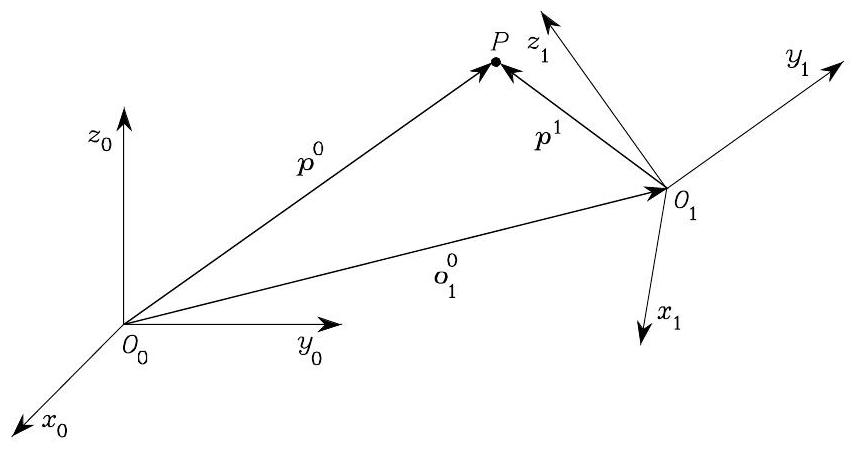
\includegraphics[max width=0.5\textwidth]{./kinematics/homogenenous_transformation}
    \caption{Representation of a point $P$ in different coordinate frames}
    \label{c1.fig.homogeneous}
\end{figure}



Consider a reference frame $O_{0}- x_{0} y_{0} z_{0}$ and another frame  $O_{1}- x_{1} y_{1} z_{1}$. Let $\boldsymbol{o}_{1}^{0}$ be the coordinate vector of the origin of Frame 1 w.r.t. Frame 0, and $\boldsymbol{R}_{1}^{0}$ be the rotation matrix of Frame 1 w.r.t. Frame 0. Let $\boldsymbol{p}^{0}$ be the coordinate vector of any point $P$ w.r.t. Frame 0, and $\boldsymbol{p}^{1}$ be the coordinate vector of the same point $P$ w.r.t. Frame 1. Then, we have the following relationship

$$
\boldsymbol{p}^{0}=\boldsymbol{o}_{1}^{0}+\boldsymbol{R}_{1}^{0} \boldsymbol{p}^{1}
$$



To achieve a compact representation, the homogeneous representation of a generic vector $\boldsymbol{p}$ is introduced:

$$
\widetilde{\boldsymbol{p}}=\left[\begin{array}{l}
\boldsymbol{p} \\
1
\end{array}\right] .
$$

Then, the above relationship can be compactly written as 

$$
\widetilde{\boldsymbol{p}}^{0}=\boldsymbol{A}_{1}^{0} \widetilde{\boldsymbol{p}}^{1}
$$

with 

$$
\boldsymbol{A}_{1}^{0}=\left[\begin{array}{cc}
\boldsymbol{R}_{1}^{0} & \boldsymbol{o}_{1}^{0} \\
\mathbf{0}^{T} & 1
\end{array}\right]
$$

which is called \emph{homogeneous transformation matrix}. All homogeneous transformation matrices belong to the \emph{Special Euclidean Group}, denoted as  $\boldsymbol{A}_{1}^{0}\in SE(3)$.

\smallskip
\noindent
The inverse transformation, 
$$
\widetilde{\boldsymbol{p}}^{1}=\boldsymbol{A}_{0}^{1} \widetilde{\boldsymbol{p}}^{0}=\left(\boldsymbol{A}_{1}^{0}\right)^{-1} \widetilde{\boldsymbol{p}}^{0}
$$
with
$$
\boldsymbol{A}_{0}^{1}=\left[\begin{array}{cc}
\boldsymbol{R}_{1}^{0 T} & -\boldsymbol{R}_{1}^{0 T} \boldsymbol{o}_{1}^{0} \\
\mathbf{0}^{T} & 1
\end{array}\right]=\left[\begin{array}{cc}
\boldsymbol{R}_{0}^{1} & -\boldsymbol{R}_{0}^{1} \boldsymbol{o}_{1}^{0} \\
\mathbf{0}^{T} & 1
\end{array}\right].
$$


Notice that for the homogeneous transformation matrix the orthogonality property does not hold; 
$$
\boldsymbol{A}^{-1} \neq \boldsymbol{A}^{T}
$$


Analogously to what presented for the rotation matrices, it is easy to verify that a sequence of coordinate transformations can be composed by the \emph{postmultiplication rule}

$$
\widetilde{\boldsymbol{p}}^{0}=\boldsymbol{A}_{1}^{0} \boldsymbol{A}_{2}^{1} \ldots \boldsymbol{A}_{n}^{n-1} \widetilde{\boldsymbol{p}}^{n}
$$

where $\boldsymbol{A}_{i}^{i-1}$ denotes the homogeneous transformation of Frame $i$ with respect to the \emph{current} Frame $i-1$.








\end{document}